\documentclass[t]{beamer}

\usetheme{TU}

\hypersetup{unicode=true,pdfcreator={},pdfproducer={}}

\usepackage{booktabs}
\usepackage{array}
\usepackage{setspace}

\title{Toolbox Workshop}
\subtitle{Nützliche Programme für Physikstudenten}
\author[Igor B.\and Kevin D.\and Christian G.\and Peter L.\and Ismo T.]{
       Igor Babuschkin%\thanks{\href{mailto:igor.babuschkin@udo.edu}{igor.babuschkin@udo.edu}}
  \and Kevin Dungs%\thanks{\href{mailto:kevin.dungs@udo.edu}{kevin.dungs@udo.edu}}
  \and Christian Gerhorst%\thanks{\href{mailto:christiangerhorst@gmail.com}{christiangerhorst@gmail.com}}
  \and Peter Lorenz%\thanks{\href{mailto:peter.lorenz@udo.edu}{peter.lorenz@udo.edu}}
  \and Ismo Toijala%\thanks{\href{mailto:ismo.toijala@udo.edu}{ismo.toijala@udo.edu}}
}
\institute[PeP et al. e.V.]{PeP et al. e.V.\thanks{\href{http://pep-dortmund.org}{pep-dortmund.org}}}
\date{September 2012}

\begin{document}
  {
    \setbeamertemplate{footline}{}
    \begin{frame}
      \titlepage
    \end{frame}
  }

  \begin{frame}{Motivation}
    \begin{itemize}
      \item Arbeitserleichterung
      \item "Gute" Tools \begin{itemize}
        \item Kein Excel!
      \end{itemize}
    \item Teamarbeit++
    \item \textit{best practices}
    \end{itemize}  
  \end{frame}

  \begin{frame}{PeP et al.}
    \begin{center}
      
\includegraphics[width=.5\paperwidth]{peplogox.png} \\
      \color{TUgreen}\textbf{\href{http://pep-dortmund.org}{www.pep-dortmund.org}}
    \end{center}
    \begin{quote}
      \begin{spacing}{1.0}
        Der Verein versteht sich als Einrichtung für Absolventen, Studierende, Mitarbeiter sowie für Freunde und Förderer der Fakultät Physik der TU Dortmund. Gegründet auf Initiative einiger Absolventen ist es seine Aufgabe, ein Netzwerk zwischen den Absolventen und der Fakultät aufzubauen.
      \end{spacing}
    \end{quote}
  \end{frame}
  

  \begin{frame}{Inhalt}
    \tableofcontents[subsectionstyle=hide]
  \end{frame}

  \section{Unix Shell}
  \subsection{Allgemeines}
    \begin{frame}{Dateisystem}
      \begin{itemize}
        \item \texttt{/} trennt Teile eines Pfads (Verzeichnisse und Dateien) (Windows: \texttt{\textbackslash})
        \item Das gesamte Dateisystem bildet \emph{einen} Baum, beginnend mit \texttt{/}
        \item Es gibt immer einen aktuellen Verzeichnis (working directory)
        \item Pfade können absolut (beginnend mit \texttt{/}) oder relativ zum aktuellen Verzeichnis angegeben werden
        \item drei spezielle Verzeichnisse:
          \begin{itemize}
            \item \texttt{.} das aktuelle Verzeichnis (oder der aktuelle im bisherigen Pfad, \texttt{a/./}~=~\texttt{a/})
            \item \texttt{..} das Oberverzeichnis des aktuellen Verzeichnisses (\texttt{a/b/../}~=~\texttt{a/})
            \item \texttt{\textasciitilde} das Heimverzeichnis (nur am Anfang eines Pfads)
          \end{itemize}
        \item Dateien, die mit \texttt{.} anfangen sind versteckt (z.B. \texttt{\textasciitilde/.vimrc})
      \end{itemize}
    \end{frame}

    \begin{frame}{Aufbau einer Eingabe}
      \texttt{\$ ls -l --all \textit{directory}\\
              \textit{output}\\
              \$}
      \begin{center}
        \begin{tabular}{>{\tt}l l}
          \toprule
          \$                 & Prompt       \\
          ls                 & Befehl       \\
          -l                 & kurze Option \\
          --all              & lange Option \\
          \textit{directory} & Argument     \\
          \textit{output}    & Ausgabe      \\
          \bottomrule
        \end{tabular}
      \end{center}
    \end{frame}

    \begin{frame}
      \begin{itemize}
        \item \texttt{\$} ist nur ein Beispiel für einen Prompt, häufig wird das aktuelle Verzeichnis und/oder andere Informationen angezeigt
        \item kurze Optionen können zusammengefasst werden (\texttt{ls~-la} = \texttt{ls -l -a} = \texttt{ls -l --all})
        \item die Reihenfolge der Optionen ist egal
        \item meistens werden mehrere Argumente (z.B. Dateien) akzeptiert
      \end{itemize}
    \end{frame}

  \subsection{Befehle}
    \begin{frame}{\texttt{man}}
      \begin{itemize}
        \item \texttt{man \textit{topic}} für manual: zeigt die Hilfe für ein Programm
        \item Beispiel: \texttt{man man}
      \end{itemize}
    \end{frame}

    \begin{frame}{\texttt{pwd}, \texttt{cd}}
      \begin{itemize}
        \item \texttt{pwd} für print working directory: zeigt das aktuelle Verzeichnis
        \item \texttt{cd \textit{directory}} für change directory: wechselt in das angegebene Verzeichnis
        \item Beispiel:\\
          \texttt{\$ pwd\\
                  /home/ismo\\
                  \$ cd ../../etc\\
                  \$ pwd\\
                  /etc\\
                  \$ cd \textasciitilde\\
                  \$ pwd\\
                  /home/ismo}
      \end{itemize}
    \end{frame}

    \begin{frame}{ls}
      \begin{itemize}
        \item \texttt{ls [\textit{directory}]} für list: zeigt den Inhalt eines Verzeichnisses an
        \item \texttt{ls -l}: zeigt mehr Informationen über Dateien und Verzeichnisse
        \item \texttt{ls -a}: zeigt auch versteckte Dateien
        \item \texttt{ls -R}: zeigt auch den Inhalt von Unterverzeichnissen
        \item alle Optionen können kombiniert werden
      \end{itemize}
    \end{frame}

    \begin{frame}
      Beispiel:\\
      \texttt{\$ ls\\
              a/  b\\
              \$ ls -l\\
              total 4.0K\\
              drwxr-xr-x 2 ismo users 4.0K Sep 15 19:52 a/\\
              -rw-r--r-- 1 ismo users \ \ \ 0 Sep 15 19:52 b\\
              \$ ls -a\\
              ./  ../  a/  b\\
              \$ ls -R\\
              .:\\
              a/  b\\
              ~\\
              ./a:\\
              c}
    \end{frame}

    \begin{frame}{\texttt{mkdir}, \texttt{touch}}
      \begin{itemize}
        \item \texttt{mkdir \textit{directory}} für make directory: erstellt ein neues Verzeichnis
        \item \texttt{mkdir -p \textit{directory}}: erstellt ein neues Verzeichnis und alle notwendigen Oberverzeichnisse
        \item \texttt{touch \textit{file}}: erstellt eine neue, leere Datei
      \end{itemize}
    \end{frame}

    \begin{frame}
      Beispiel:\\
      \texttt{\$ ls\\
              \$ mkdir a\\
              \$ mkdir b/c\\
              mkdir: cannot create directory ‘b/c’: No such file or directory\\
              \$ mkdir -p b/c\\
              \$ touch b/file\\
              \$ ls -R\\
              .:\\
              a/  b/\\
              ~\\
              ./a:\\
              ~\\                  
              ./b:\\
              c/ file\\
              ~\\
              ./b/c:}
    \end{frame}

    \begin{frame}{\texttt{cp}, \texttt{mv}, \texttt{rm}, \texttt{rmdir}}
      \begin{itemize}
        \item \texttt{cp \textit{source} \textit{destination}} für copy: kopiert eine Datei
        \item \texttt{cp -r \textit{source} \textit{destination}}: kopiert ein Verzeichnis rekursiv
        \item das Ziel kann ein Verzeichnis oder der exakte Pfad sein
        \item \texttt{mv \textit{source} \textit{destination}} für move: verschiebt order benennt eine Datei um
        \item Ziel kann wir bei \texttt{cp} sein
        \item \texttt{rm \textit{file}} für remove: löscht eine Datei
        \item \texttt{rm -r \textit{file}}: löscht ein Verzeichnis rekursiv
        \item \texttt{rmdir \textit{directory}} für remove directory: löscht ein leeres Verzeichnis
        \item \texttt{rm -r} kann statt \texttt{rmdir} verwendet werden
      \end{itemize}
    \end{frame}

    \begin{frame}
      Beispiel:\\
      \texttt{\$ ls\\
              a\\
              \$ cp a b\\
              \$ ls\\
              a  b\\
              \$ mv b c\\
              \$ ls\\
              a  c\\
              \$ rm a\\
              \$ ls\\
              c}
    \end{frame}

    \begin{frame}{\texttt{cat}, \texttt{less}, \texttt{grep}}
      \begin{itemize}
        \item \texttt{cat [\textit{file}]} für concatenate: gibt den Inhalt einer (oder mehr) Dateien aus
        \item \texttt{less [\textit{file}]} (besser als \texttt{more}): zeigt eine Datei in einer navigablen Form an
        \item \texttt{grep \textit{pattern} [\textit{file}]} für ???: sucht nach einem Muster
        \item \texttt{grep -i \textit{pattern} [\textit{file}]}: ignoriert Groß- und Kleinschreibung
        \item \texttt{grep -r \textit{pattern} \textit{directory}}: sucht rekursiv in allen Dateien
      \end{itemize}
    \end{frame}

    \begin{frame}{Allgemeines}
      \begin{itemize}
        \item pipes\\
        \item ctrl-c\\
        \item ctrl-d\\
        \item .., .\\
        \item >, >>, <\\
        \item glob (*, ...)
      \end{itemize}
    \end{frame}

  \section{git}
\begin{frame}{git}
  \begin{center}
    
\includegraphics[width=100px]{../Notes/img/git.pdf}
  \end{center}
  \tableofcontents[sectionstyle=show/hide,
                   subsectionstyle=show/show/hide,
                   subsubsectionstyle=show/show/show]
\end{frame}

\subsection{Warum?}
\begin{frame}{Warum?}
  \begin{block}{Warum Versionskontrolle?}
    \begin{itemize}
      \item Backup
      \item vereinfachte Kollaboration
      \item Protokollierung
    \end{itemize}
  \end{block}
  \begin{block}{Warum Git?}
    \begin{itemize}
      \item \textit{distributed} Version Control System
      \item sehr schnell
      \item setzt sich momentan durch
    \end{itemize}
  \end{block}
\end{frame}

\subsection{Hoster}
\begin{frame}{Hoster}
  \begin{itemize}
    \item $
      \begin{array}{l}
        
\includegraphics[height=18px]{../Notes/img/octocat.jpg}
      \end{array} $ \textbf{Github} (\url{https://github.com/})\\
      kostenlose öffentliche Repositories, gute UI
    \item $
      \begin{array}{l}
        
\includegraphics[height=18px]{../Notes/img/bitbucket.png}
      \end{array} $ \textbf{Bitbucket} (\url{https://bitbucket.org})\\
      kostenlose private Repositories
  \end{itemize}
\end{frame}

\begin{frame}{Übersicht}
\end{frame}

\subsection{Befehle}
\begin{frame}{Repository erstellen}
  \begin{itemize}
    \item \texttt{git init}  Erzeugt ein leeres Repository im jetzigen Ordner
    \item \texttt{git clone [\textit{url}]} Kopiert ein Repository aus dem Internet
  \end{itemize}
\end{frame}

\begin{frame}{Informationen abrufen}
  \begin{itemize}
    \item \texttt{git status} Zeigt an, welche Dateien geändert wurden und welche bereits im Index sind
    \item \texttt{git log}    Zeigt alle gespeicherten Commits an
  \end{itemize}
\end{frame}

\begin{frame}{Dateien zum Index hinzufügen}
  \begin{itemize}
    \item \texttt{git add} Fügt eine Datei oder einen Ordner (mit Inhalt) zum Index hinzu
    \item \texttt{git rm}  Löscht eine Datei aus dem Ordner und schreibt die Löschung in den Index
    \item \texttt{git mv}  Genauso, aber die Datei wird verschoben
  \end{itemize}
\end{frame}

\begin{frame}{Commits erstellen}
  \begin{itemize}
    \item \texttt{git commit} Speichert die Änderungen im Index als Commit ab
  \end{itemize}
\end{frame}

\begin{frame}{Änderungen runter-/hochladen}
  \begin{itemize}
    \item \texttt{git pull} Neue Commits runterladen\\
                            Falls man noch neue lokale Commits hat führt git einen \textit{merge} durch
    \item \texttt{git push} Neue Commits hochladen\\
                            Geht nur, wenn keine neuen Commits im zentralen Repository sind\\
                            Wenn ja, erst einmal \texttt{git pull} verwenden
  \end{itemize}
\end{frame}

\begin{frame}{Manuell mergen}
  \begin{itemize}
    \item \texttt{git mergetool} Startet ein Programm, mit dem man manuell mergen kann, falls die Automatik nicht funktioniert
  \end{itemize}
\end{frame}

  \section{Python}
\begin{frame}{Python}
  \begin{center}
    
\includegraphics[width=140px]{img/python.png} \\
    \color{TUgreen}\textbf{\href{http://python.org}{www.python.org}}
  \end{center}
  \begin{quote}
    \begin{spacing}{1.0}
      Python is a programming language that lets you work more quickly and integrate your systems more effectively.
      You can learn to use Python and see almost immediate gains in productivity and lower maintenance costs.
    \end{spacing}
  \end{quote}
\end{frame}

\begin{frame}{Python ist...}
  \begin{itemize}
    \item […] eine Programmiersprache.
    \item […] einfach!
    \item […] sehr mächtig.
    \item […] universell einsetzbar.
  \end{itemize}
  \begin{center}
    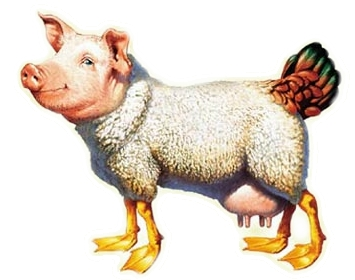
\includegraphics[width=120px]{img/eierlegendewollmilchsau.jpg}\\
    \tiny\texttt{\href{http://xn--sptzlemitsoss-cfb.de/wp-content/uploads/2012/07/eierlegendewollmilchsau.jpg}{http://xn--sptzlemitsoss-cfb.de/wp-content/uploads/2012/07/eierlegendewollmilchsau.jpg}}\normalsize
  \end{center}
\end{frame}

\begin{frame}[fragile]{Ein kleines Beispiel}
  \vspace{-1em}
  \begin{columns}
    \begin{column}{0.5\textwidth}
      \begin{exampleblock}{C++}
        \begin{minted}[fontsize=\footnotesize]{c++}
#include <iostream>
using namespace std;
int main(int argc, char *argv[])
{
    cout << "Hello, World!" << endl;
    return 0;
}
        \end{minted}
      \end{exampleblock}
    \end{column}
    \begin{column}{0.5\textwidth}
      \begin{exampleblock}{Python}
        \begin{minted}[fontsize=\footnotesize]{python}
print("Hello, World!")
        \end{minted}
      \end{exampleblock}
    \end{column}
  \end{columns}
\end{frame}

\begin{frame}{Python}
  \tableofcontents[sectionstyle=show/hide,
                   subsectionstyle=show/show/hide,
                   subsubsectionstyle=show/show/show]
\end{frame}

\subsection{IPython}
\begin{frame}{IPython}
  \begin{center}
    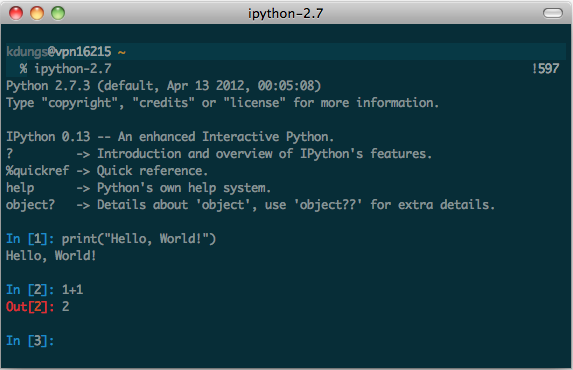
\includegraphics[width=300px]{img/ipython.png}
  \end{center}
\end{frame}

\subsection{Syntax}
\begin{frame}{Syntax}
  \begin{block}{Blöcke}
    \begin{itemize}
      \item Durch Einrückung!
      \item 4 Leerzeichen (/1 Tab)
    \end{itemize}
  \end{block}
  \begin{block}{Semikolons}
  \begin{itemize}
    \item Gibt es prinzipiell
    \item Sind am Zeilenende aber nicht notwendig
  \end{itemize}
  \end{block}
\end{frame}

\begin{frame}[fragile]{Variablen}
  \begin{itemize}
    \item Dynamische Typisierung
    \item Keine explizite Deklaration 
  \end{itemize}
  \begin{spacing}{1.0}
    \begin{exampleblock}{Beispiel}
      \begin{minted}{python}
In [1]: a = 1

In [2]: b = 2

In [3]: name = "Kääähbiiin"

In [4]: a, b, name
Out[4]: (1, 2, 'Kääähbiiin')
      \end{minted}
    \end{exampleblock}
  \end{spacing}  
\end{frame}

\begin{frame}{Datenstrukturen}
  \begin{itemize}
    \item bool (\texttt{True}, \texttt{False})
    \item int, float, long, complex
    \item string (\texttt{'foo'}, \texttt{"bar"})
    \item Iteratoren, Generatoren, Sequenzen, …
  \end{itemize}
\end{frame}

\begin{frame}[fragile]{Datenstrukturen}
  \begin{block}{Praktische Typen}
    \begin{itemize}
      \item[\texttt{()}] Tupel
      \item[\texttt{[]}] Liste
      \item[\texttt{\{\}}] Dictionary 
    \end{itemize}
  \end{block}
  \vspace{.5em}
  \begin{spacing}{1.0}
    \begin{exampleblock}{Zum Beispiel}
      \begin{minted}{python}
In [9]: cities = ['Dortmund', 'Hamburg', 'Berlin']

In [10]: cities[0]
Out[10]: 'Dortmund'
      \end{minted}
    \end{exampleblock}
  \end{spacing}
\end{frame}

\begin{frame}[fragile]{Mehr Beispiele}
  \begin{minted}{python}
In [1]: teams = {
   ...:         'BVB': "BV Borussia Dortmund 09",
   ...:         'S04': "FC Schalke 04",
   ...:         'FCB': "FC Bayern München"
   ...: }

In [2]: teams['BVB']
Out[2]: 'BV Borussia Dortmund 09'
  \end{minted}
\end{frame}

\begin{frame}[fragile]{Operatoren}
  \begin{spacing}{1.0}
    \begin{block}{Arithmetische Operatoren}
      \begin{minted}{python}
+, -, *, /, %, **, //
      \end{minted}
    \end{block}
    \begin{block}{Zuweisungsoperatoren}
      \begin{minted}{python}
=, +=, -=, *=, /=, %=, **=, //=
      \end{minted}
    \end{block}
    \begin{block}{Vergleichsoperatoren}
      \begin{minted}{python}
==, !=, <, <=, >, >=
      \end{minted}
    \end{block}
  \end{spacing}
\end{frame}

\begin{frame}[fragile]{Operatoren}
  \begin{spacing}{1.0}
    \begin{block}{Logische Operatoren}
      \begin{minted}{python}
and, or, not
      \end{minted}
    \end{block}
    \begin{block}{Identitätsoperatoren}
      \begin{minted}{python}
is, is not
      \end{minted}
    \end{block}
    \begin{block}{Operatoren für Sequenzen}
      \begin{minted}{python}
in, not in
      \end{minted}
    \end{block}
  \end{spacing}
\end{frame}

\begin{frame}[fragile]{Kontrollstrukturen}
  \begin{spacing}{1.0}
    \begin{block}{if}
      \begin{minted}{python}
if condition:
    # do something
elif other_condition:
    # or do something else
else:
    # or something else
      \end{minted}
    \end{block}
    \begin{block}{case}
      gibt es \emph{nicht}!
    \end{block}
  \end{spacing}
\end{frame}

\begin{frame}[fragile]{Schleifen}
  \begin{block}{while}
    \begin{minted}{python}
while condition:
    # do something
    \end{minted}
  \end{block}
  \begin{block}{for}
  \begin{itemize}
   \item \texttt{for … in}
   \item agiert immer auf \emph{Sequenzen}!
  \end{itemize}
  \end{block}
\end{frame}

\begin{frame}[fragile]{for - Beispiele}
\vspace{-1em}
\begin{spacing}{1.0}
\begin{columns}
    \begin{column}{0.4\paperwidth}
      \begin{exampleblock}{Listen}
        \begin{minted}{python}
for city in cities:
    print(city)
    
Dortmund
Hamburg
Berlin
        \end{minted}
      \end{exampleblock}
    \end{column}
    \begin{column}{.4\paperwidth}
      \begin{exampleblock}{Range}
        \begin{minted}{python}
for i in range(0, 10):
    print(i)
    
0
1
2
3
…
        \end{minted}
      \end{exampleblock}
    \end{column}
  \end{columns}
\end{spacing}
\end{frame}

\begin{frame}{Funktionen}
  \begin{block}{Aufrufe}
  \end{block}
  \begin{block}{def}
  \end{block}
\end{frame}

\begin{frame}{Module}
  import, from, as
\end{frame}

\begin{frame}[fragile]{Und ohne IPython?}
  \begin{itemize}
    \item Dateiendung \texttt{.py}
    \item Aufruf per \texttt{python3 dateiname.py}
    \item \texttt{print()}-Funktion 
  \end{itemize}
\end{frame}

\subsection{Bibliotheken}
\subsubsection{NumPy}
\begin{frame}{NumPy}
\end{frame}

\subsubsection{SciPy}
\begin{frame}{SciPy}
\end{frame}

\subsubsection{matplotlib}
\begin{frame}{matplotlib}
\end{frame}

\subsubsection{PyLab}
\begin{frame}{PyLab}
\end{frame}

\end{document}
